\documentclass[Main]{subfiles}
\begin{document}

\chapter{GUI}

The GUI was created using Matlab GUIDE. The GUI utilizes the encoder function described in section \ref{sec:EncImpl} and the decoder described in sections \ref{sec:decImplOv} through \ref{sec:decoderImpl}. The implementation details of the GUI are not in the scope of this report, but the source code is attached as appendix \ref{App:SourceCode}.
The GUI is shown in figure \ref{fig:meggittGUI}.

\begin{figure}[h]
    \centering
    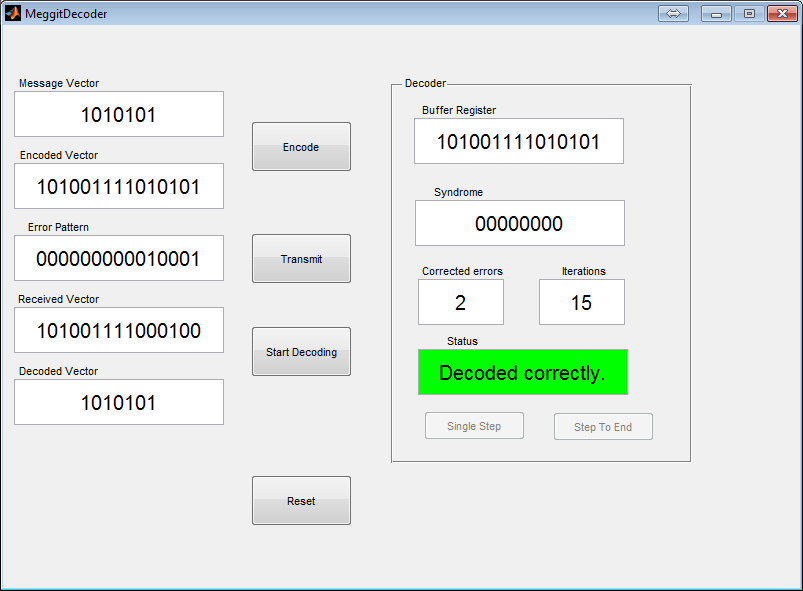
\includegraphics[width=0.7\textwidth]{figures/gui}
    \caption{Meggitt decoder GUI}
    \label{fig:meggittGUI}
\end{figure}

The following is a brief description of the elements of the GUI. Input to the encoding and decoding process is given using the input textboxes \textit{Message Vector} and \textit{Error Pattern}. The \textit{Encode} button invokes the encoder to create the \textit{Encoded Vector}. The \textit{Transmit} button applies the \textit{Error Pattern} to create the \textit{Received Vector}. The \textit{Start Decoding} button initializes the decoder with the \textit{Recieved Vector}, and calc 


\end{document} 